	\section*{Exercice 4 (5 points)}
	
	\subsection*{1. Étudier le signe de la fonction \(P\) définie sur \(\mathbb{R}\) par \(P(x) = x^2 + 4x + 3\).}
	
\[ P(x) = x^2 + 4x + 3 = (x + 2)^2 - 4 + 3 = (x + 2)^2 - 1 = (x + 3)(x + 1). \]
On sait que \(P(x) > 0\), sauf sur l’intervalle \(\left] -3, -1 \right[\) (-3 et -1 étant les racines du trinôme).

	\subsection*{2. Montrer que pour tout réel \(x\) de l’intervalle \(\left] -2, +\infty \right[\),
		\[ f'(x) = \dfrac{P(x)}{(x + 2)^2}, \]
		où \(f'\) est la fonction dérivée de \(f\).}
	
	Pour \(x > -2\), \(f\) est dérivable et sur \(\left] -2, +\infty \right[\) :
	\[ f'(x) = \dfrac{(2x + 1)(x + 2) - (x^2 + x - 1)}{(x + 2)^2} = \dfrac{2x^2 + 4x + x + 2 - x^2 - x + 1}{(x + 2)^2} = \dfrac{x^2 + 4x + 3}{(x + 2)^2} = \dfrac{P(x)}{(x + 2)^2}. \]
	
	\subsection*{3. Étudier le signe de \(f'(x)\) sur \(\left] -2, +\infty \right[\) et construire le tableau de variations de la fonction \(f\) sur \(\left] -2, +\infty \right[\).}
Comme \((x + 2)^2 > 0\) sur \(\left] -2, +\infty \right[\), le signe de \(f'(x)\) est celui du numérateur \(P(x)\) étudié à la question 1.
Donc sur \(\left] -2, -1 \right[\), \(f'(x) < 0\) : la fonction est décroissante et sur \(\left] -1, +\infty \right[\) la fonction \(f\) est croissante.
	
	\begin{center}
	\begin{tikzpicture}[double distance=2pt]
		\tkzTabInit{$x$/1,$f'(x)$/1,$f(x)$/2}{$-\infty$,$-1$, $+\infty$}
		\tkzTabLine{,-,z, +}
		\tkzTabVar{+/,-/$-1$,+/}
	\end{tikzpicture}
\end{center} 
	
	\subsection*{4. Donner le minimum de la fonction \(f\) sur \(\left] -2, +\infty \right[\) et la valeur pour laquelle il est atteint (on donnera les valeurs exactes).}
	
	D’après la question précédente \(f(-1) = \dfrac{1 - 1 - 1}{-1 + 2} = -1\) est le minimum de la fonction \(f\) sur \(\left] -2, +\infty \right[\).
	
	\subsection*{5. Déterminer le coefficient directeur de la tangente \(T\) à la courbe \(C_f\) au point d’abscisse 2.}
	
	Le coefficient directeur de la tangente \(T\) à la courbe \(C_f\) au point d’abscisse 2 est le nombre dérivé \(f'(2)\) :
	\[ f'(2) = \dfrac{4 + 8 + 3}{(2 + 2)^2} = \dfrac{15}{16} = 0,9375. \]
	
